\chapter{Dominio de problema}
\label{cap:dominio}

\section{Problema}
Investigadores del Departamento de Física de la Universidad de Santiago de Chile pertenecientes al CEDENNA se encuentran estudiando los efectos de aplicar ciertos campos magnéticos a nano-estructuras cristalinas, con propiedades físicas definidas. Los resultados de estas simulaciones pueden ser aplicados a la producción de nuevos dispositivos magnéticos o para el grabado de datos magnético de alta densidad  \citep{asymmetricMagneticDots}.

\section{Estructuras cristalinas}
Las nano-estructuras estudiadas son de tipo cristalinas, las que pueden ser divididas en celdas unitarias de distintos tipos  según la distribución de sus átomos. Las 3 estructuras más usadas son el cubo simple (\emph{SC} o \emph{Simple Cubic}), cubo centrado en su cuerpo (\emph{BCC} o \emph{Body-centered Cubic}) y cubo centrado en sus caras (\emph{FCC} o \emph{Face-centered cubic}) \citep{ITC213}.

En las estructuras cristalinas la dimensión física de las aristas está dada por el parámetro llamado \emph{Lattice Parameter} o Parámetro de Red. Como en este caso solo se trabajará con estructuras cúbicas todas las aristas tendrán la misma dimensión, por lo que nos referiremos a este parámetro como \emph{Lattice Constant} o Constante de Red.

Para cada átomo de una estructura cristalina se puede identificar un conjunto de átomos que componen la vecindad, es decir, son los átomos que están a menor distancia de este. Dependiendo del tipo de celdas unitarias se define un algoritmo para encontrar los vecinos e identificar el número máximo de vecinos que pueden ser encontrados.

Dependiendo del tipo de estructura se puede encontrar patrones de periodicidad entre ellas, es decir, que cada cierto número de capas se repita la misma distribución de átomos.

\subsection{Cubo simple (SC)}
\label{structureSC}
Esta es la estructura cristalina más simple, donde en cada vértice podemos encontrar una partícula. Luego la distancia entre dos átomos vecinos es siempre la constante de red (ver figura \ref{SimpleCubic}). Como en cada vértice de la estructura se unen 8 celdas unitarias, cada cubo tiene $1/8$ de partícula, luego cada celda tiene $1/8 \cdot 8 = 1$ átomo en total.

En el caso del cubo simple la vecindad de cada átomo está compuesta a lo más por otros 6 átomos, los que están en dirección a cada una de las aristas que componen el vértice donde se encuentra la partícula.

El cubo simple tiene una periodicidad de 1, es decir, todas las capas tienen la misma distribución de átomos.

\begin{figure}[ht]
  \centering
  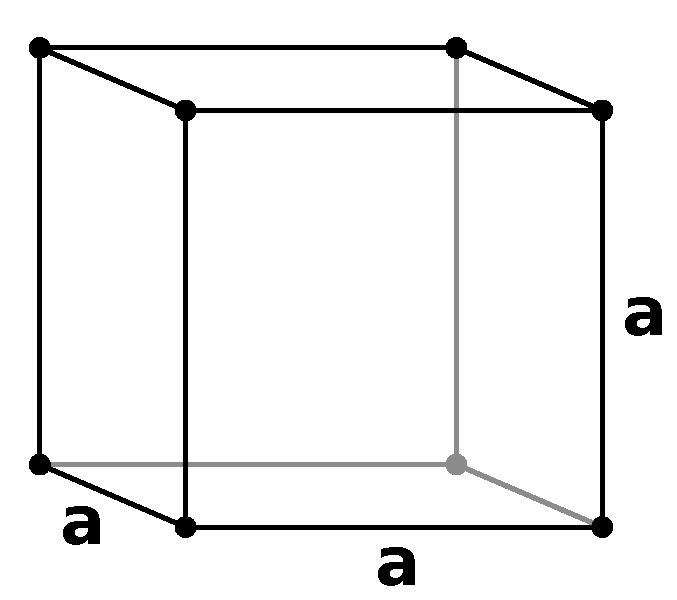
\includegraphics[scale=.6]{images/SimpleCubic}
  \caption{\em Cubo simple, con constante de red $a$}
  \label{SimpleCubic}
\end{figure}


\subsection{Cubo centrado en su cuerpo (BCC)}
\label{structureBCC}
Una estructura cristalina de cubos centrados en su cuerpo se caracteriza porque en cada una de sus celdas unitarias se puede encontrar, además de los átomos en sus vértices, un átomo en su centro (ver figura \ref{BodyCenteredCubic}). De esta forma cada una de sus celdas tiene $1/8$ de átomo en cada uno de sus vértices, más un átomo en su centro, resultando en $1/8 \cdot 8 + 1 = 2$ átomos en total.

A diferencia de un cubo simple, la vecindad de un átomo en BCC está compuesta por:

\begin{itemize}
  \item Para el caso de un átomo ubicado en un vértice, las partículas centrales de cada uno de los cubos que componen dicho vértice.
  \item Para el caso de un átomo ubicado en el centro de una celda unitaria, las partículas ubicadas en cada uno de los vértices de dicha celda.
\end{itemize}

En ambos casos el número máximo de partículas en una vecindad es de 8.

La periodicidad de capas de una estructura compuesta por cubos centrados en su cuerpo es de 2, es decir, cada 2 capas se repetirá la distribución de átomos.

\begin{figure}[ht]
  \centering
  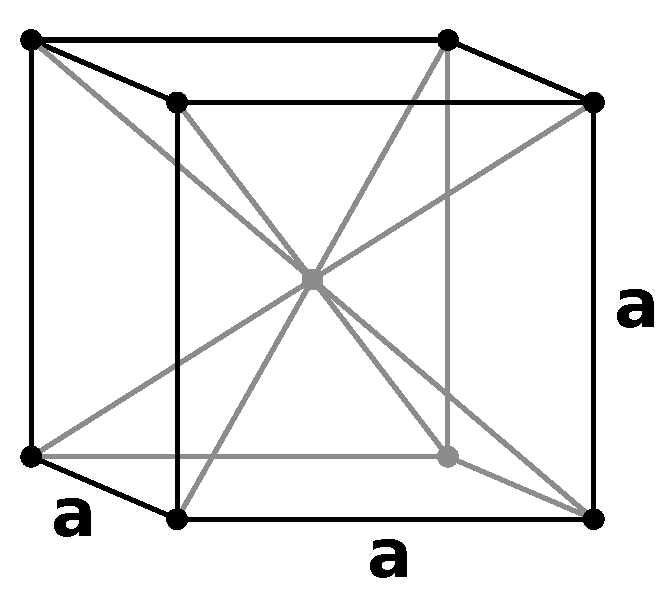
\includegraphics[scale=.6]{images/BodyCenteredCubic}
  \caption{\em Cubo centrado en su cuerpo, con constante de red $a$}
  \label{BodyCenteredCubic}
\end{figure}


\subsection{Cubo centrado en sus caras (FCC)}
\label{structureFCC}
En el caso de las estructuras cristalinas compuesta por cubos centrados en sus caras se puede distinguir átomos en cada uno de sus vértices y átomos en cada una de las caras de cada cubo (ver figura \ref{FaceCenteredCubic}). Como el átomo de una cara es compartido por 2 cubos, cada uno de ellos contiene $1/2$ de éste, y por lo tanto cada celda unitaria contiene $1/8 \cdot 8 + 1/2 \cdot 6 = 4$ átomos en total.

La vecindad de un átomo FCC está compuesta por:

\begin{itemize}
  \item Las partículas de cada cara que esté compuesta por una de las aristas que conforman el vértice, para el caso de un átomo ubicado en ese punto
  \item En el caso de las partículas que se encuentran en una cara, todos los átomos ubicados en las caras formados por las aristas que componen la cara del átomo inicial (2 caras por arista), además de los átomos que están en los vértices que componen la cara inicial
\end{itemize}

De las reglas anteriores se puede inferir que el tamaño máximo de una vecindad es de 12 átomos.

Para las estructuras formadas por cubos centrados en sus caras se identifica una periodicidad de 2, es decir, al igual que en el caso de los cubos centrados en su cuerpo, cada 2 capas se repite la distribución atómica.

\begin{figure}[ht]
  \centering
  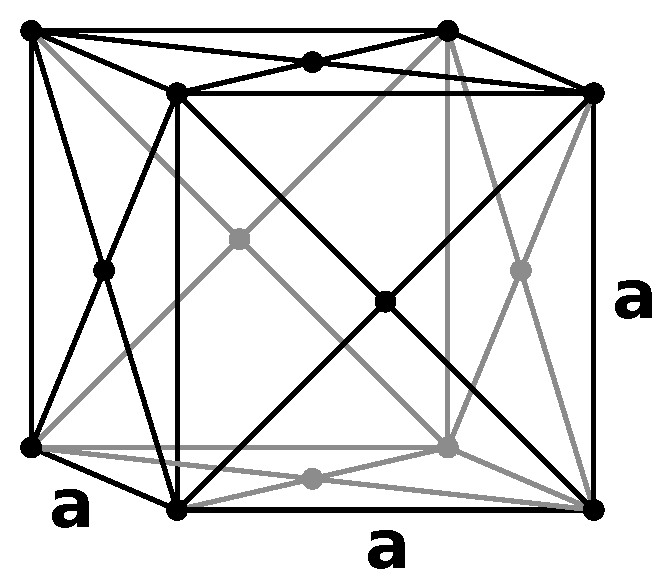
\includegraphics[scale=.6]{images/FaceCenteredCubic}
  \caption{\em Cubo centrado en sus caras}
  \label{FaceCenteredCubic}
\end{figure}

\section{Escalamiento}

A pesar de la gran capacidad de procesamiento de los computadores actuales aún resulta inconveniente simular los sistemas con sus características reales, debido a la gran cantidad de átomos que deberían ser simulados, que dependiendo del objeto pueden ser de orden de magnitud $10^8$. Para esto los científicos han propuesto un método de escalamiento de las configuraciones que les permita reducir significativamente el número de átomos y obtener soluciones válidas \citep{PhysRevB.71.094435}. El método fue validado mediante un diagrama de fase magnético para un cilindro con ciertas características materiales y físicas, en función de su diámetro y altura. En este diagrama notaron que un diagrama modificado (o escalado) $J' = J \cdot X$, con la constante de escalamiento $X < 1$ se puede obtener modificando las dimensiones del cilindro en base a la siguiente relación:

\begin{center}
$Longitud' = Longitud \cdot X ^ \eta$ , con $\eta = 0.55$
\end{center}

\noindent
donde Longitud puede ser cualquiera de las 3 dimensiones, alto, ancho o profundidad.

Con esta relación de escalamiento las relaciones magnéticas entre los átomos se mantienen intactas, y las simulaciones entregan resultados válidos.

EL diseño de configuraciones escaladas en base a las dimensiones reales se realiza de la siguiente dorma. Dada la constante de red, el tipo de estructura cristalina y el número de capas deseado, se calcula la altura escalada del objeto mediante:

\begin{center}
    $$Altura' = \dfrac{Capas * Constante\ de\ Red}{Periodicidad\ de\ la\ estructura\ cristalina}$$
\end{center}

Luego, y conociendo la altura real, se calcula la constante de escalamiento con la siguiente ecuación:

\begin{center}
$X = \bigg( \dfrac{Altura'}{Altura} \bigg)^{\nicefrac{1}{\eta}}$
\end{center}

Finalmente, las otras dos dimensiones escaladas pueden obtenerse mediante:

\begin{center}
$$Ancho' = X^\eta \cdot Ancho$$
$$Profundidad' = X^\eta \cdot Profundidad$$
\end{center}

\section{Método Monte Carlo}

El Método Monte Carlo es un método estadístico (no determinista) propuesto por Nicholas Metropolis et al en 1949, mientras trabajaba en el desarrollo de la Bomba Atómica en el Laboratorio nacional de Los Alamos en EEUU, que permite obtener soluciones aproximadas a problemas muy difíciles de solucionar de forma matemática (determinista) debido a su magnitud o complejidad, para esto se basa en la aleatoriedad. Primero se debe determinar que condiciones se deben cumplir para que cierto caso a probar sea válido, estos pueden ser, por ejemplo, un set de ecuaciones con múltiples parámetros o resultados de interacciones entre un cierto grupo de partículas, luego genera sets de prueba aleatorios que pueden cumplir o no las condiciones definidas, luego de una gran cantidad de iteraciones se pueden usar los resultados válidos para obtener conclusiones. De cierta forma se experimenta teóricamente las distintas combinaciones de factores que afectan un problema definido.

Dependiendo de donde se desea aplicar el método es posible que no sea necesario que los números generados para las pruebas no sean realmente aleatorios, si no que, en general, solo se necesita que sean lo suficientemente aleatorios, para esto existen diversas pruebas estadísticas con las que se puede validar, como que con una gran cantidad de elementos generados no exista un patrón claro de generación y que estos estén distribuidos de forma uniforme.

\section{Aplicación del Método Monte Carlo al problema}

Para esta investigación los científicos aplicarán el Método Monte Carlo usando las siguientes condiciones \citep{TesisAllende}:

\begin{itemize}
 \item Se selecciona una partícula $i$ al azar y se calcula su energía $E_1 = E(\vec{m}_i)$
 \item Se modifica la dirección del vector de magnetización de la partícula $i$ al azar y se calcula la nueva energía $E_2 = E(\vec{m}'_i)$
 \item Se considera válido el cambio de $\vec{m}_i$ a $\vec{m}'_i$ si se cumple alguna de las siguientes condiciones
 \begin{itemize}
  \item $E_2$ es menor que $E_1$
  \item $E_2$ es mayor que $E_1$ y se cumple con la relación $\exp(-\beta(E_2 - E_1)) > \varepsilon$, donde $\beta = (kT)^-1$ siendo $k$ la constante de Boltzmann, $T$ la temperatura \citep{newmanb99} y $\varepsilon$ un número aleatorio entre 0 y 1
 \end{itemize}
\end{itemize}

En caso de que las condiciones no se satisfagan se considera inválido el cambio y se rechaza, es decir, se conserva $\vec{m}_i$.

Analizaremos los parámetros de simulación de uno de los casos estudiado por los científicos usando el Método Monte Carlo \citep{asymmetricMagneticDots}, para esto trabajaremos con un \emph{dot} circular, con diámetro $d$ = 80 nm y altura $h$ = 20 nm. Como fue explicado anteriormente resulta prácticamente imposible analizar estos objetos en tamaño real, por lo que deben ser escalados lo suficiente para poder ejecutar los cálculos usando la tecnología disponible actualmente sin perder sus características magnéticas como el desarrollo de \emph{vortex} magnéticos, para esto se usará un factor de escalamiento $X = 0.01 - 0.001$, esto se logra usando $\eta \approx 0.55 - 0.57$ y por supuesto escalando las dimensiones iniciales de forma $d' = dx^\eta$ y $h' = hx^\eta$.

Para elegir la nueva orientación del campo magnético se usará un generador aleatorio con una probabilidad $p = min[1, \exp(-\Delta E/k_BT')]$, donde $\Delta E$ es el cambio de energía debido a la reorientación del spin, $k_B$ es la constante de Boltzmann y $T' = Tx$, con $T = 10K$.

Inicialmente se aplica un campo hacia el eje $X$ de magnitud $H=5.5kOe$ y se analizaran pasos de $\Delta H = 0.1kOe$, es decir, para completar una curva de histéresis son necesarios 110 pasos de $\Delta H$. En cada uno de estos pasos se analizará el campo magnético del \emph{dot}, ejecutando 3.500 pasos Monte Carlo por cada $\Delta H$, por lo que la cantidad de pasos para esta simulación es de $110 \cdot 3500 = 385000$ de forma de completar la curva de histéresis.

En cada uno de estos pasos es necesario hacer un cálculo de energía del \emph{dot}.

Este proceso completo se repite varias veces con distintas semillas para el generador aleatorio de números, para así validar el resultado.

\section{Cálculo de Energía}

Para calcular la energía total $E_{tot}$ de un \emph{dot} se usa la siguiente ecuación:

\begin{center}
  $$E_{tot} = \frac{1}{2} \sum_{i \neq j} (E_{ij} - J_{ij} \hat{\mu}_i \cdot \hat{\mu}_j) + E_H$$
\end{center}

\noindent
donde $E_{ij}$ es la energía dipolar dada por

\begin{center}
  $$E_{ij} = [\vec{\mu}_i \cdot \hat{\mu}_j - 3(\vec{\mu}_i \cdot \hat{n}_{ij})(\vec{\mu}_j \cdot \hat{n}_{ij})]/ r^3_{ij}$$
\end{center}

\noindent
con $r_{ij}$ la distancia entre los vectores de magnetización $\vec{\mu}_i$  y $\vec{\mu}_j$ y $\hat{n}_{ij}$ el vector unitario en la dirección que conecta los dos vectores de magnetización. $\hat{\mu}_i$ es un vector unitario en la dirección de $\vec{\mu}_i$ y $E_H = - \sum_i \vec{\mu}_i \cdot \vec{H}$ representa la energía Zeeman para un campo $\vec{H}$ aplicado hacia el eje x.

$J_{ij}$ es la interacción de canje magnético entre $i$ y $j$, es decir, como sus campos magnéticos internos se afectan entre ellos, para este caso se asumirá que $J_{ij} = 0$ para dos átomos que no son vecinos. Como en el caso de dos partículas vecinas es necesario calcular esta interacción, al momento de ejecutar la simulación es necesario saber, para cada átomo, quienes componen su vecindad.
